\section{Montag}

\begin{tcolorbox}
    Das ausschlaggebende Kriterium für die Verwendung von \code{notify()} / \code{notifyAll()} ist nicht die Anzahl der wartenden Threads in den Warteschlangen eines passiven Objektes, sondern die Anzahl der Threads, die ihre \textit{while-wait-Schleife} verlassen können.
\end{tcolorbox}

\begin{figure}
    \centering
    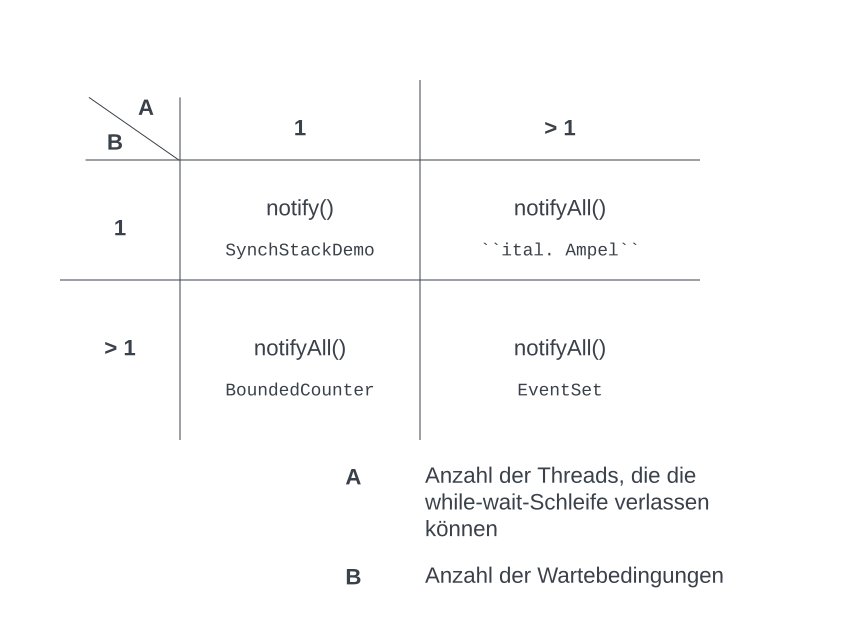
\includegraphics[scale=0.5]{chapters/Anhang/Präsenzphase/img/notifynotifyall}
    \caption{Merkregel für die Verwendung von notify()/notifyAll() mit den besprochenen Aufgaben als Beispiel. I.d.R. wird notify() nur genutzt, wenn es nur einen Thread gibt, der die while-wait-Schleife verlassen kann, und es gleichzeitig nur eine Wartebedingung gibt. (Quelle: eigene)}
    \label{fig:notifynotifyall}
\end{figure}
